%% =========================================================================
%% Section 5: Primary Regression Findings
%% =========================================================================

\section{Primary Regression Findings}

\subsection{Cognitive Impairment: Attenuation by Adult Socioeconomic Attainment}
Table~\ref{tab:cog_reg} presents sequential survey-weighted modified Poisson regressions for low memory-orientation performance ($N = 57{,}245$). 

\begin{table}[!htbp]
\centering
\small
\caption{\textbf{Sequential Survey-Weighted Modified Poisson Regressions for Cognitive Impairment ($\mathbf{N=57{,}245}$).}}
\label{tab:cog_reg}
\resizebox{\textwidth}{!}{%
\begin{tabular}{lcccc}
\toprule
\textbf{Childhood Exposure Parameter} & \textbf{Model 0: Crude} & \textbf{Model A: Demog.+State} & \textbf{Model B: +Adult SES (Primary)} & \textbf{Model C: +Adult Health} \\
\midrule
Childhood SES: Average & 0.97 (0.82--1.15) \textit{p}=0.711 & 0.98 (0.84--1.14) \textit{p}=0.777 & 0.80 (0.70--0.91) \textit{p}$<$0.001 & 0.80 (0.71--0.91) \textit{p}$<$0.001 \\
Childhood SES: Poor & 1.61 (1.33--1.96) \textit{p}$<$0.001 & 1.36 (1.16--1.59) \textit{p}$<$0.001 & \textbf{0.93 (0.82--1.05) \textit{p}=0.241} & 0.91 (0.81--1.03) \textit{p}=0.148 \\
\midrule
Childhood bedridden $\ge$1 month & 0.90 (0.77--1.06) \textit{p}=0.222 & 0.94 (0.81--1.09) \textit{p}=0.404 & 1.00 (0.86--1.18) \textit{p}=0.947 & 0.99 (0.84--1.16) \textit{p}=0.868 \\
\midrule
Childhood health: Fair/Poor/Very poor & 0.97 (0.81--1.17) \textit{p}=0.773 & 0.97 (0.85--1.12) \textit{p}=0.719 & 0.95 (0.82--1.10) \textit{p}=0.487 & 0.95 (0.82--1.09) \textit{p}=0.458 \\
Childhood health: Poor/Very poor (orig) & 1.15 (0.86--1.53) \textit{p}=0.338 & 1.02 (0.78--1.34) \textit{p}=0.856 & 1.07 (0.81--1.41) \textit{p}=0.629 & 0.99 (0.75--1.31) \textit{p}=0.953 \\
\bottomrule
\end{tabular}%
}
\end{table}

The regression progression demonstrates a striking life-course attenuation story:
\begin{enumerate}
    \item \textbf{Crude Association (Model 0):} In unadjusted analyses, adults raised in poor childhood homes had a \textbf{61\% higher prevalence} of cognitive impairment compared to those from well-off childhoods ($\text{PR} = 1.61$, 95\% CI: 1.33--1.96, $p < 0.001$).
    \item \textbf{Demographic Adjustment (Model A):} Accounting for age, gender, rural/urban sector, caste, and 36 state fixed effects partially attenuates this association to a 36\% elevation ($\text{APR} = 1.36$, 95\% CI: 1.16--1.59, $p < 0.001$).
    \item \textbf{Full Attenuation via Adult SES (Model B):} When adult educational attainment (7 categorical levels) and household per capita consumption expenditure (5 MPCE quintiles) are introduced, the childhood socioeconomic disparity \textbf{evaporates completely} ($\text{APR} = 0.93$, 95\% CI: 0.82--1.05, $p = 0.241$). Adults who grew up in poor households have no higher rate of memory-orientation impairment than their well-off peers, once their adult schooling and household wealth are equalized.
    \item \textbf{Early Health Null on Memory/Orientation:} Neither general childhood health ($\text{APR} = 0.95, p = 0.487$) nor prolonged childhood bedridden illness ($\text{APR} = 1.00, p = 0.947$) showed any association with binary cognitive impairment across any model specification.
\end{enumerate}

\subsection{Continuous Memory-Orientation Score: Linear Survey Regression}
Table~\ref{tab:cog_cont} evaluates continuous memory and orientation scores (0--28 points) using survey-weighted linear regression (WLS with design-based standard errors) across all sequential model specifications.

\begin{table}[!htbp]
\centering
\small
\caption{\textbf{Continuous Memory and Orientation Score Regressions (Linear Survey OLS, $\hat{\beta}$ Point Differences, $\mathbf{N=57{,}245}$).}}
\label{tab:cog_cont}
\resizebox{\textwidth}{!}{%
\begin{tabular}{llcccc}
\toprule
\textbf{Exposure Parameter} & \textbf{Contrast Level} & \textbf{Model 0: Crude} & \textbf{Model A: Demog.+State} & \textbf{Model B: +Adult SES} & \textbf{Model C: +Adult Health} \\
\midrule
Childhood SES & Average (vs. Well-off) & $-0.31$ ($-0.58$ to $-0.04$) & $-0.35$ ($-0.58$ to $-0.13$) & $+0.12$ ($-0.10$ to $+0.33$) & $+0.13$ ($-0.09$ to $+0.35$) \\
              & Poor (vs. Well-off)    & $-1.65$ ($-1.95$ to $-1.34$) & $-1.28$ ($-1.54$ to $-1.02$) & \textbf{$-0.32$ ($-0.56$ to $-0.09$)} & $-0.25$ ($-0.48$ to $-0.01$) \\
\midrule
Childhood Health & Fair/Poor (vs. Good) & $-0.02$ ($-0.43$ to $+0.39$) & $-0.05$ ($-0.29$ to $+0.18$) & $+0.01$ ($-0.23$ to $+0.25$) & $+0.04$ ($-0.19$ to $+0.27$) \\
                 & Poor/Very poor (orig) & $-0.45$ ($-0.88$ to $-0.04$) & $-0.23$ ($-0.59$ to $+0.13$) & $-0.26$ ($-0.63$ to $+0.10$) & $-0.04$ ($-0.41$ to $+0.33$) \\
\midrule
Childhood Bedridden & Yes (vs. No)       & $+0.14$ ($-0.25$ to $+0.53$) & $+0.02$ ($-0.19$ to $+0.23$) & $-0.15$ ($-0.35$ to $+0.05$) & $-0.10$ ($-0.30$ to $+0.10$) \\
\bottomrule
\end{tabular}%
}
\end{table}

In unadjusted linear models, poor childhood SES was associated with a $-1.65$ point deficit ($p < 0.001$) on the 28-point scale. Demographic and geographic adjustment reduced this penalty to $-1.28$ points. Introducing adult education and MPCE consumption quintiles (Model B) attenuated this penalty by \textbf{75\%}, leaving a small, residual deficit of \textbf{$-0.32$ points} (95\% CI: $-0.56$ to $-0.09$, $p = 0.008$). Although statistically significant due to the immense statistical power of 57,245 respondents, this residual penalty represents barely 1.1\% of the scale range. As detailed in our domain decomposition analysis in Section 6, this modest deficit is driven entirely by episodic word recall rather than orientation awareness.

\subsection{Depressive Symptoms: Enduring, Non-Attenuated Disparities}
In sharp, profound contrast to cognitive impairment, Table~\ref{tab:dep_reg} demonstrates that early-life disadvantage exerts \textbf{enduring, persistent associations with late-life depressive symptoms} that cannot be erased by adult educational or financial success.

\begin{table}[!htbp]
\centering
\small
\caption{\textbf{Sequential Survey-Weighted Modified Poisson Regressions for Depressive Symptoms ($\mathbf{N=62{,}047}$).}}
\label{tab:dep_reg}
\resizebox{\textwidth}{!}{%
\begin{tabular}{lcccc}
\toprule
\textbf{Childhood Exposure Parameter} & \textbf{Model 0: Crude} & \textbf{Model A: Demog.+State} & \textbf{Model B: +Adult SES (Primary)} & \textbf{Model C: +Adult Health} \\
\midrule
Childhood SES: Average & 1.10 (0.94--1.30) \textit{p}=0.233 & 1.20 (1.01--1.44) \textit{p}=0.039 & 1.15 (0.99--1.33) \textit{p}=0.072 & 1.14 (0.99--1.32) \textit{p}=0.071 \\
Childhood SES: Poor & 1.17 (1.00--1.37) \textit{p}=0.044 & 1.31 (1.09--1.58) \textit{p}=0.004 & \textbf{1.21 (1.03--1.42) \textit{p}=0.019} & 1.15 (0.99--1.34) \textit{p}=0.068 \\
\midrule
Childhood bedridden $\ge$1 month & 1.14 (1.01--1.29) \textit{p}=0.037 & 1.14 (1.01--1.27) \textit{p}=0.034 & \textbf{1.16 (1.05--1.28) \textit{p}=0.004} & 1.11 (1.01--1.23) \textit{p}=0.029 \\
\midrule
Childhood health: Fair/Poor/Very poor & 1.33 (1.20--1.47) \textit{p}$<$0.001 & 1.21 (1.08--1.36) \textit{p}=0.002 & \textbf{1.20 (1.07--1.34) \textit{p}=0.002} & 1.19 (1.06--1.33) \textit{p}=0.002 \\
Childhood health: Poor/Very poor (orig) & 1.51 (1.26--1.80) \textit{p}$<$0.001 & 1.42 (1.21--1.67) \textit{p}$<$0.001 & \textbf{1.42 (1.21--1.66) \textit{p}$<$0.001} & 1.25 (1.06--1.48) \textit{p}=0.008 \\
\bottomrule
\end{tabular}%
}
\end{table}

Key insights from Table~\ref{tab:dep_reg} include:
\begin{enumerate}
    \item \textbf{Childhood Poor Health Leaves Lasting Psychological Marks:} In primary Model B, older adults who experienced poor or fair health up to age 16 have a \textbf{20\% higher prevalence} of late-life depressive symptoms ($\text{APR} = 1.20$, 95\% CI: 1.07--1.34, $p = 0.002$), adjusting for demographics, state fixed effects, adult education, and MPCE. When using the narrower published definition (Poor/Very poor), the risk elevation is even higher at \textbf{42\%} ($\text{APR} = 1.42$, 95\% CI: 1.21--1.66, $p < 0.001$).
    \item \textbf{Childhood Poverty Persists:} Growing up in a financially poor family confers a \textbf{21\% higher prevalence} of depressive symptoms in later life ($\text{APR} = 1.21$, 95\% CI: 1.03--1.42, $p = 0.019$), independent of current adult wealth.
    \item \textbf{Prolonged Bedridden Illness:} Having been bedridden for a month or more in childhood elevates late-life depression by \textbf{16\%} ($\text{APR} = 1.16$, 95\% CI: 1.05--1.28, $p = 0.004$).
    \item \textbf{Resistance to Downstream Adult Health Controls (Model C):} Even after further conditioning on current adult chronic physical diseases (hypertension, diabetes, heart disease, stroke, lung disease) and self-rated health, poor childhood health ($\text{APR} = 1.19, p = 0.002$) and childhood bedridden illness ($\text{APR} = 1.11, p = 0.029$) remain statistically significant.
\end{enumerate}

\subsubsection{Sex-Stratified Heterogeneity in Childhood Adversity and Depression}
Sex-stratified models (mutually adjusted, Model B) reveal an important gendered asymmetry in who carries the childhood poverty scar into later life. Among women ($n = 33{,}226$), poor childhood SES was associated with a \textbf{23\% higher prevalence} of depressive symptoms ($\text{APR} = 1.23$, 95\% CI: 1.01--1.49, $p = 0.037$), with the association maintained after full adjustment for adult education and wealth. Among men ($n = 28{,}821$), the corresponding estimate was 14\% ($\text{APR} = 1.14$, 95\% CI: 0.96--1.35, $p = 0.146$) and did not reach statistical significance.

Similarly, poor childhood health was significantly associated with late-life depressive symptoms among women ($\text{APR} = 1.21$, 95\% CI: 1.09--1.35, $p < 0.001$) but was attenuated and non-significant among men ($\text{APR} = 1.15$, 95\% CI: 0.99--1.34, $p = 0.075$). Childhood bedridden illness displayed a parallel pattern ($\text{APR} = 1.10, p = 0.069$ in women vs. $\text{APR} = 1.13, p = 0.198$ in men). In stark contrast, cognitive impairment showed no sex divergence: both women ($\text{APR} = 0.97, p = 0.712$) and men ($\text{APR} = 0.83, p = 0.147$) showed complete attenuation of early SES disparities to the null. These findings confirm that older women disproportionately bear the long-term affective burden of early-life deprivation in India.

Figure~\ref{fig:forest_plot} displays the sequential forest plot, vividly illustrating the divergence: cognitive disparities collapse to the vertical null line ($\text{APR} = 1.0$) upon adjusting for adult schooling, while depressive symptom disparities remain stubbornly elevated to the right of the null line across all specifications.

\begin{figure}[!htbp]
    \centering
    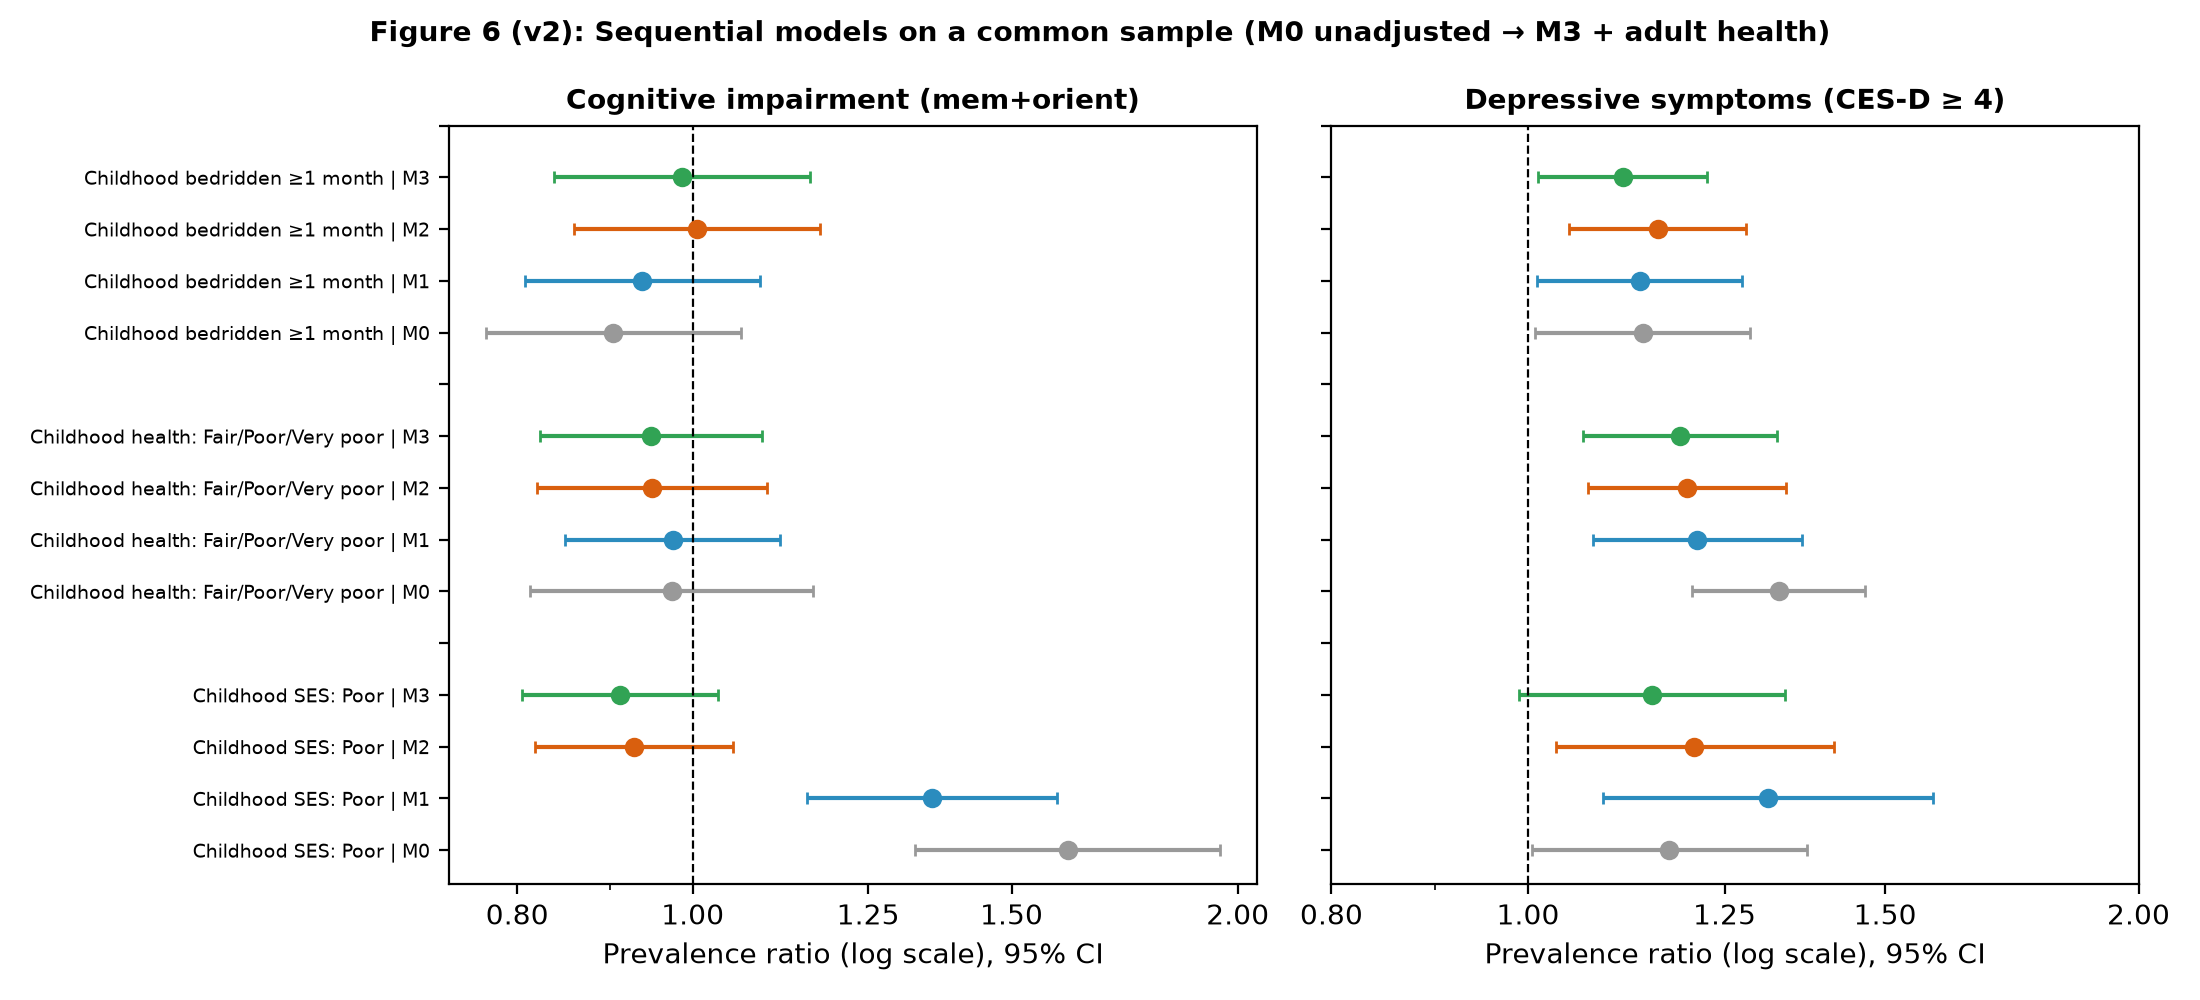
\includegraphics[width=0.92\textwidth]{figures/figure6v2_forest_sequential.png}
    \caption{\textbf{Sequential Model Forest Plots for Cognitive Impairment and Depressive Symptoms.} Contrasts the attenuation of cognitive disparities toward the null line ($\text{APR} = 1.0$) against the persistent elevation of depressive symptom disparities across Models 0 through C.}
    \label{fig:forest_plot}
\end{figure}

\subsection{Mutually Adjusted Models and Cumulative Adversity Dose-Response}
Table~\ref{tab:mutual_models} evaluates models where all three early-life exposures were entered simultaneously into the regression equation, testing whether they represent redundant manifestations of general disadvantage or distinct independent risks.

\begin{table}[!htbp]
\centering
\small
\caption{\textbf{Mutually Adjusted Childhood Models and Cumulative Disadvantage Score across Sequential Model Specifications.}}
\label{tab:mutual_models}
\resizebox{\textwidth}{!}{%
\begin{tabular}{llcc}
\toprule
\textbf{Model Hierarchy} & \textbf{Childhood Exposure Parameter} & \textbf{Prevalence Ratio (95\% CI)} & \textbf{\textit{p}-value} \\
\midrule
\multicolumn{4}{l}{\textbf{Panel A: Cognitive Impairment ($N = 57{,}245$)}} \\
\midrule
Model A: Demographics + State & Childhood SES: Average & 0.98 (0.84 -- 1.14) & $0.792$ \\
Model A: Demographics + State & Childhood SES: Poor & 1.36 (1.15 -- 1.60) & $<0.001$ \\
Model A: Demographics + State & Childhood health: Fair/Poor/Very poor & 0.97 (0.84 -- 1.12) & $0.681$ \\
Model A: Demographics + State & Childhood bedridden $\ge 1$ month & 0.94 (0.81 -- 1.10) & $0.430$ \\
\addlinespace
Model B: + Adult SES (Primary) & Childhood SES: Average & 0.80 (0.70 -- 0.91) & $<0.001$ \\
Model B: + Adult SES (Primary) & Childhood SES: Poor & 0.93 (0.82 -- 1.06) & $0.277$ \\
Model B: + Adult SES (Primary) & Childhood health: Fair/Poor/Very poor & 0.95 (0.82 -- 1.10) & $0.533$ \\
Model B: + Adult SES (Primary) & Childhood bedridden $\ge 1$ month & 1.01 (0.86 -- 1.18) & $0.941$ \\
\addlinespace
Model C: + Adult Health Pathway & Childhood SES: Poor & 0.91 (0.81 -- 1.04) & $0.171$ \\
Model C: + Adult Health Pathway & Childhood health: Fair/Poor/Very poor & 0.95 (0.83 -- 1.10) & $0.514$ \\
Model C: + Adult Health Pathway & Childhood bedridden $\ge 1$ month & 0.99 (0.84 -- 1.17) & $0.892$ \\
\addlinespace
Model B: Cumulative Index & Per additional childhood adversity (0 to 3) & 1.05 (0.99 -- 1.12) & $0.071$ \\
\midrule
\multicolumn{4}{l}{\textbf{Panel B: Depressive Symptoms ($N = 62{,}047$)}} \\
\midrule
Model A: Demographics + State & Childhood SES: Average & 1.18 (1.00 -- 1.39) & $0.044$ \\
Model A: Demographics + State & Childhood SES: Poor & 1.29 (1.08 -- 1.54) & $0.005$ \\
Model A: Demographics + State & Childhood health: Fair/Poor/Very poor & 1.19 (1.05 -- 1.34) & $0.005$ \\
Model A: Demographics + State & Childhood bedridden $\ge 1$ month & 1.10 (0.97 -- 1.25) & $0.147$ \\
\addlinespace
Model B: + Adult SES (Primary) & Childhood SES: Average & 1.13 (0.98 -- 1.29) & $0.090$ \\
Model B: + Adult SES (Primary) & Childhood SES: Poor & \textbf{1.19 (1.02 -- 1.38)} & \textbf{$0.026$} \\
Model B: + Adult SES (Primary) & Childhood health: Fair/Poor/Very poor & \textbf{1.18 (1.05 -- 1.32)} & \textbf{$0.006$} \\
Model B: + Adult SES (Primary) & Childhood bedridden $\ge 1$ month & \textbf{1.12 (1.00 -- 1.26)} & \textbf{$0.044$} \\
\addlinespace
Model C: + Adult Health Pathway & Childhood SES: Poor & 1.13 (0.98 -- 1.31) & $0.089$ \\
Model C: + Adult Health Pathway & Childhood health: Fair/Poor/Very poor & 1.17 (1.05 -- 1.31) & $0.006$ \\
Model C: + Adult Health Pathway & Childhood bedridden $\ge 1$ month & 1.08 (0.97 -- 1.21) & $0.157$ \\
\addlinespace
\textbf{Model B: Cumulative Index} & \textbf{Per additional childhood adversity (0 to 3)} & \textbf{1.114 (1.070 -- 1.160)} & \textbf{$<0.001$} \\
\bottomrule
\end{tabular}%
}
\end{table}

In Model B mutually adjusted depression models:
\begin{itemize}
    \item Poor childhood SES ($\text{APR} = 1.19$, 95\% CI: 1.02--1.38, $p = 0.026$), poor childhood health ($\text{APR} = 1.18$, 95\% CI: 1.05--1.32, $p = 0.006$), and bedridden illness ($\text{APR} = 1.12$, 95\% CI: 1.00--1.26, $p = 0.044$) maintained \textbf{independent, non-overlapping associations}. Experiencing childhood health shocks carries an emotional cost that is distinct from growing up in family poverty.
    \item \textbf{Dose-Response Gradients:} The Cumulative Childhood Adversity Index demonstrates a highly significant, linear dose-response relationship: \textbf{each additional childhood adversity is associated with an 11.4\% higher prevalence of late-life depressive symptoms} ($\text{APR} = 1.114$, 95\% CI: 1.070--1.160, $p < 0.001$).
\end{itemize}

\subsection{Social Mobility and the Persistence of Early-Life Scars}
A fundamental sociological question asks: \textit{Does upward social mobility in adulthood erase the health penalties of a disadvantaged childhood, or do early scars remain permanently etched into biological and psychological functioning?}

To test this directly, we constructed four mutually exclusive \textbf{intergenerational mobility trajectories} by crossing childhood socioeconomic status with adult household consumption expenditure (MPCE quintiles 1--2 as low adult SES; quintiles 3--5 as high adult SES):
\begin{itemize}
    \item \textbf{Persistently Affluent (Reference):} Non-poor childhood $\rightarrow$ high adult consumption ($N = 23{,}289$ in cognitive sample; $N = 24{,}643$ in depression sample).
    \item \textbf{Downwardly Mobile:} Non-poor childhood $\rightarrow$ low adult consumption ($N = 12{,}330$ cognitive; $N = 13{,}336$ depression).
    \item \textbf{Upwardly Mobile:} Poor childhood $\rightarrow$ high adult consumption ($N = 11{,}451$ cognitive; $N = 12{,}544$ depression).
    \item \textbf{Persistently Poor:} Poor childhood $\rightarrow$ low adult consumption ($N = 10{,}175$ cognitive; $N = 11{,}524$ depression).
\end{itemize}

Table~\ref{tab:social_mobility} presents sequential modified Poisson models using mobility trajectory as the primary exposure, alongside standardized predicted prevalences evaluated under Model B.

\begin{table}[!htbp]
\centering
\small
\caption{\textbf{Social Mobility Trajectories, Cognitive Impairment, and Depressive Symptoms (Prevalence Ratios and Model B Standardized Prevalences).}}
\label{tab:social_mobility}
\resizebox{\textwidth}{!}{%
\begin{tabular}{llcccc}
\toprule
\textbf{Outcome Domain} & \textbf{Mobility Trajectory Group} & \textbf{Model 0: Crude PR} & \textbf{Model A: Demog. PR} & \textbf{Model B: +Schooling PR} & \textbf{Model B Prev. (\%, 95\% CI)} \\
\midrule
\textbf{Cognitive Impairment} & Persistently Affluent (Ref.) & 1.000 & 1.000 & 1.000 & 10.86 (10.21--11.80) \\
($N = 57{,}245$)              & Downwardly Mobile            & 1.525 (1.329--1.751)$^{***}$ & 1.427 (1.273--1.600)$^{***}$ & 1.184 (1.072--1.308)$^{***}$ & 12.86 (12.07--13.99) \\
                              & Upwardly Mobile              & 1.763 (1.537--2.023)$^{***}$ & 1.505 (1.332--1.700)$^{***}$ & 1.196 (1.072--1.333)$^{**}$ & 12.98 (12.20--14.17) \\
                              & Persistently Poor            & 2.184 (1.901--2.510)$^{***}$ & 1.752 (1.562--1.964)$^{***}$ & 1.278 (1.149--1.421)$^{***}$ & 13.87 (13.03--15.08) \\
\midrule
\textbf{Depressive Symptoms}  & Persistently Affluent (Ref.) & 1.000 & 1.000 & 1.000 & 26.58 (25.28--28.45) \\
($N = 62{,}047$)              & Downwardly Mobile            & 1.076 (0.996--1.163)$^{\dagger}$ & 1.104 (1.015--1.201)$^{*}$   & 1.064 (0.975--1.161)         & 28.28 (26.79--30.19) \\
                              & Upwardly Mobile              & 1.100 (1.011--1.198)$^{*}$   & 1.147 (1.037--1.268)$^{**}$  & 1.099 (0.995--1.214)$^{\dagger}$ & \textbf{29.21 (27.55--31.39)} \\
                              & Persistently Poor            & 1.116 (1.025--1.215)$^{*}$   & 1.177 (1.070--1.296)$^{***}$ & 1.105 (0.998--1.223)$^{\dagger}$ & \textbf{29.37 (27.72--31.39)} \\
\bottomrule
\multicolumn{6}{l}{\footnotesize $^{***}\ p < 0.001$, $^{**}\ p < 0.01$, $^{*}\ p < 0.05$, $^{\dagger}\ p < 0.10$. Model B adjusts for age, sex, residence, caste, marital status, state FE, and education (excluding MPCE collinear with trajectory).} \\
\end{tabular}%
}
\end{table}

\begin{figure}[!htbp]
    \centering
    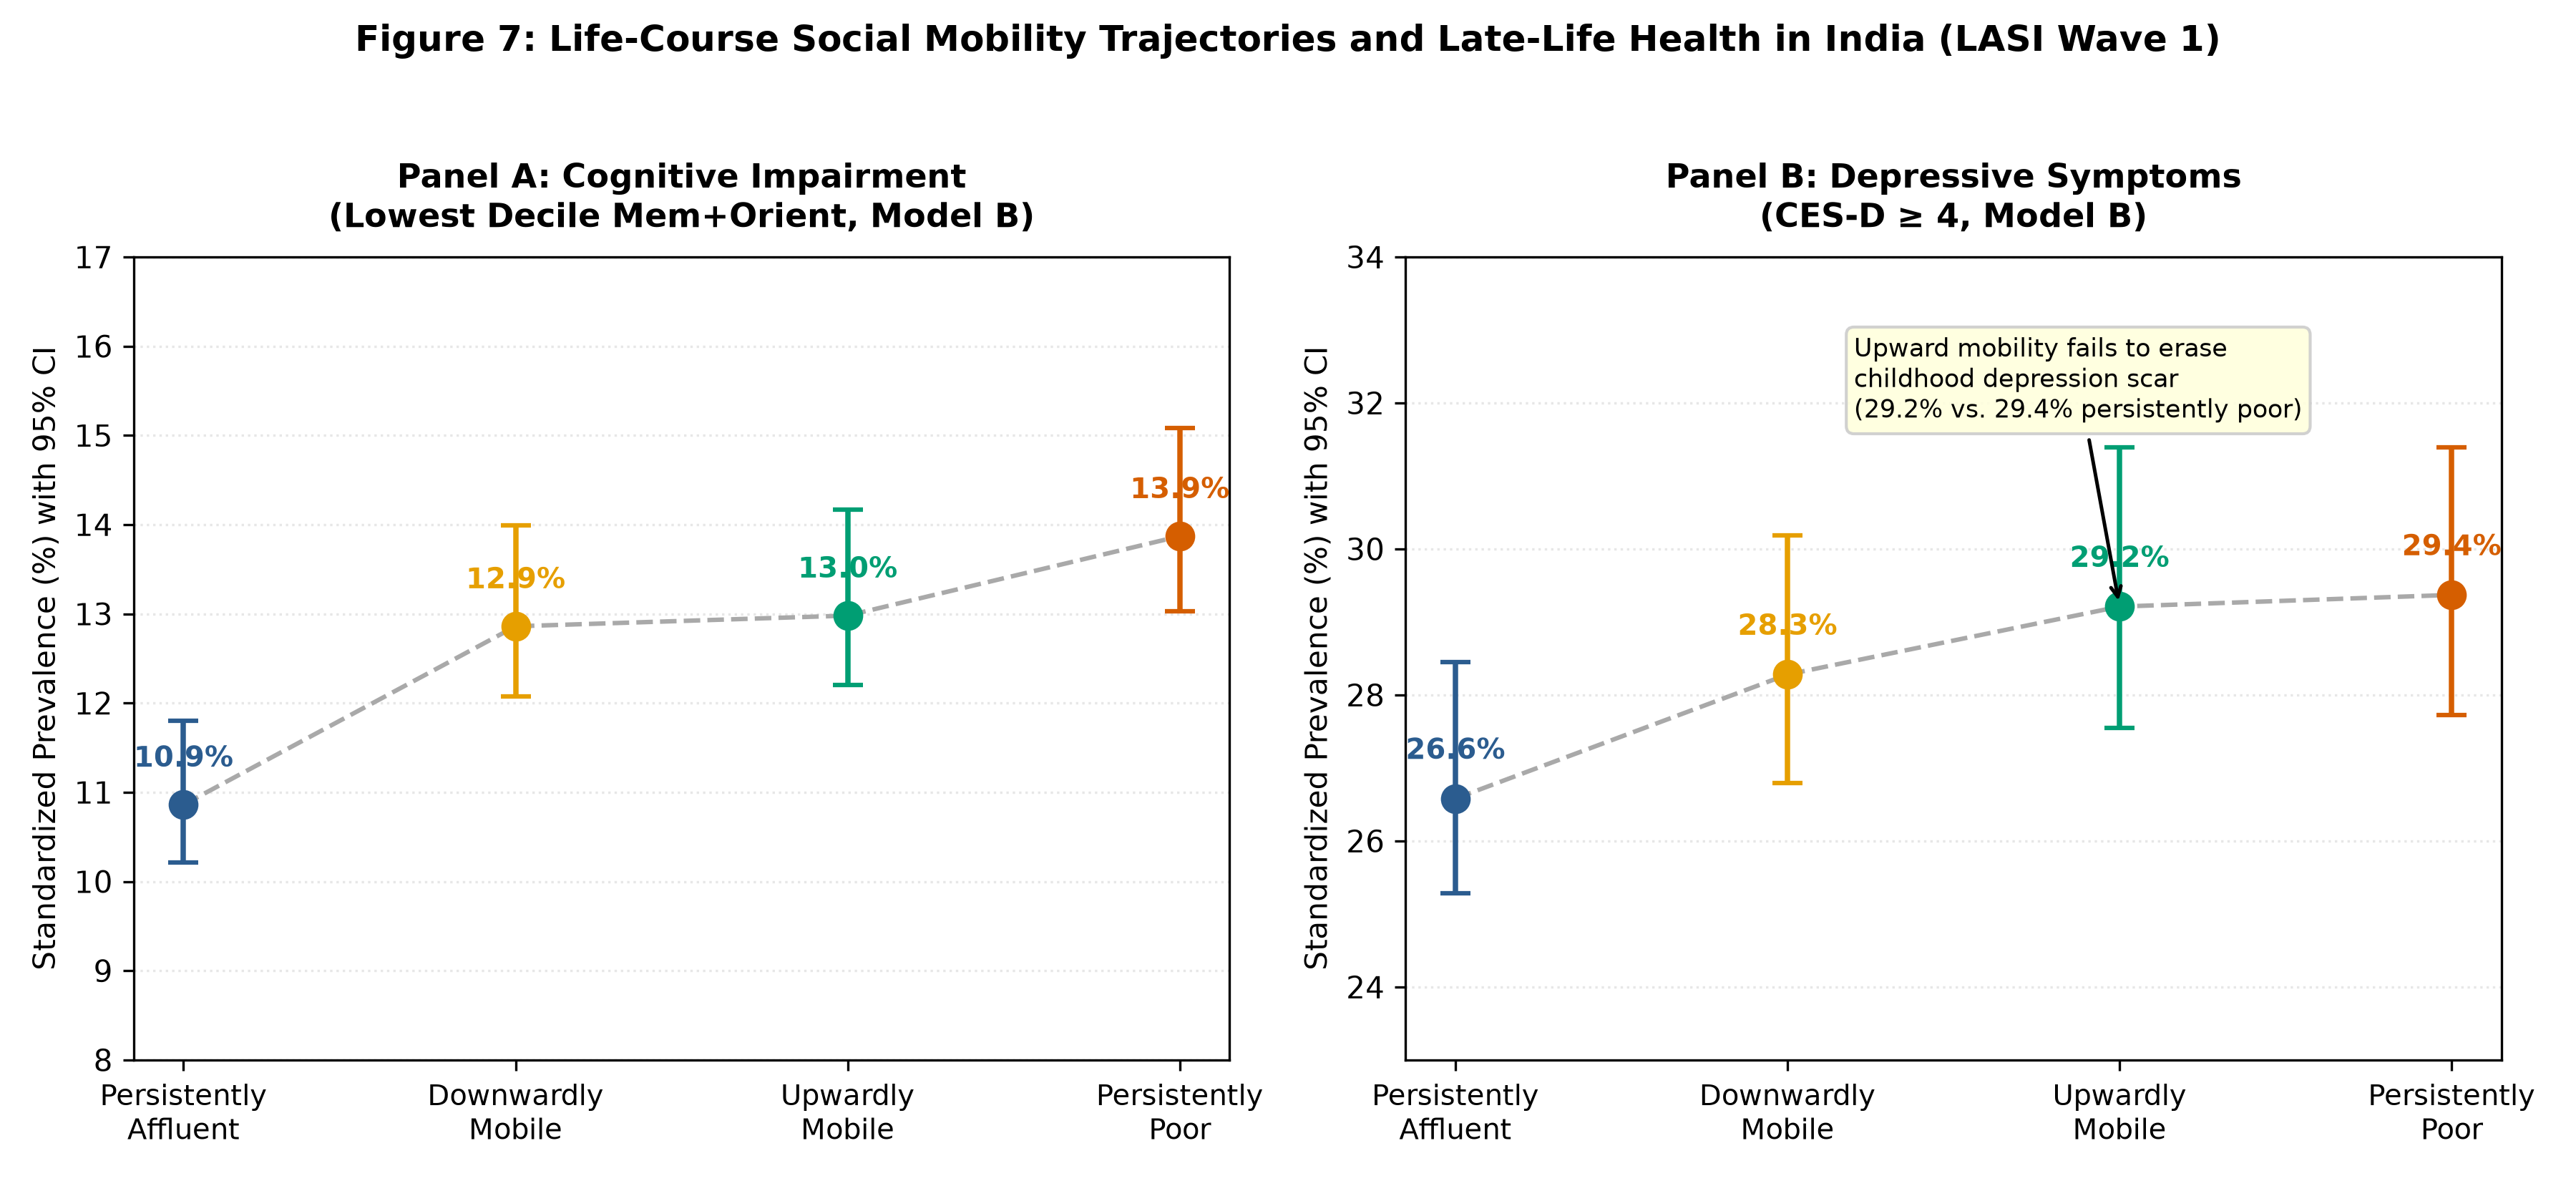
\includegraphics[width=0.95\textwidth]{figures/figure7_social_mobility.png}
    \caption{\textbf{Life-Course Social Mobility Trajectories and Late-Life Health in India.} Adjusted standardized prevalences (\%) with 95\% confidence intervals evaluated under Model B across four intergenerational trajectories. Note that upward mobility substantially narrows cognitive deficits (Panel A) but leaves late-life depression risk completely unattenuated (Panel B: 29.2\% vs. 29.4\% among persistently poor).}
    \label{fig:social_mobility}
\end{figure}

The mobility analysis uncovers a critical sociological asymmetry illustrated in Figure~\ref{fig:social_mobility}:
\begin{enumerate}
    \item \textbf{Cognitive Disadvantage is Responsive to Mobility:} For cognitive impairment, crude disparities follow a steep status hierarchy: Persistently Affluent (10.86\%) $<$ Downwardly Mobile (12.86\%) $\approx$ Upwardly Mobile (12.98\%) $<$ Persistently Poor (13.87\%). Individuals who start life in poverty but achieve upward consumption mobility see their impairment penalty drop from $\text{PR} = 1.76$ (crude) to $\text{APR} = 1.20$ after accounting for schooling. Upward mobility narrows the gap with the persistently affluent group by over 60\%, demonstrating that acquired educational and material resources actively protect cognitive reserve.
    \item \textbf{Depression Scars Resist Upward Mobility:} In marked contrast, upward mobility fails to heal childhood psychological scars. Older adults who achieved upward mobility display a standardized depression prevalence of \textbf{29.21\%} (95\% CI: 27.55\%--31.39\%)—a figure virtually identical to the \textbf{29.37\%} observed among those who remained persistently poor throughout their lives, and significantly higher than the 26.58\% observed among the persistently affluent. Moving up the economic ladder in adulthood does not erase the neuro-affective vulnerabilities forged in an impoverished childhood.
\end{enumerate}
